% ===== Section 2: "Carrots and sticks" (compliance techniques and why they work) (~18 min) + break =====
\partaccent{butter}
\topicopener{carrot}{Համոզելու հնարքներ}{Գազար ու փայտ}{Ինչպես ենք կառավարում ուրիշներին, ու ինչպես են կառավարում մեզ}{smug}

% Burnett buys a car (and takes his dad)
\begin{frame}{Բըրնեթը մեքենա է գնում}
  \begin{columns}[c]
    \begin{column}{0.55\textwidth}
      \begin{itemize}
        \item Այնքան մեքենա ես տեսնում, որ սկսում ես մտածել՝ բակում ձիու համար տեղ կլինի՞
        \item Անիվներին քացի ես տալիս, որ գիտակ երևաս։ \textbf{Կոշիկիդ ծայրը կարո՞ղ է ռետին վերլուծել}
        \item<2-> Իսկ ամենավատը վաճառողներն են. կեղծ ընկերականություն, «պետք է մենեջերին հարցնեմ»
      \end{itemize}
    \end{column}
    \begin{column}{0.41\textwidth}
      \centering
      \bigemoji[1.1cm]{car}\ \bigemoji[1.1cm]{moneybag}\par\medskip
      \onslide<3->{%
      \begin{card}[colback=butter!45!cream]
        Դրա համար Բըրնեթը միշտ \textbf{հորն} է տանում։ Հոր մարտավարությունը. հայհոյել վաճառողներին ու հանցագործ անվանել, մինչև գինն իջեցնեն։\par\smallskip
        Ոչ նրբանկատ, բայց \textbf{արդյունավետ} \emoji{angry}
      \end{card}}
    \end{column}
  \end{columns}
\end{frame}

% Why do sales tricks work at all?
\begin{frame}{Ինչու են հնարքներն աշխատում}
  \begin{columns}[c]
    \begin{column}{0.58\textwidth}
      \begin{itemize}
        \item Գնորդները բոլորովին տարբեր են, բայց նույն հնարքները աշխատում են \textbf{ամենուր}
        \item Կան վարքեր, որոնք մեծացնում են \textbf{զիջողականությունը} (compliance). մարդը համաձայնում է դիմացինի խնդրանքին
        \item<3-> Բայց մարդուն ամբողջությամբ կառավարել չի կարելի, ինչ էլ որ պնդեն «գայթակղության գուրուները»
      \end{itemize}
    \end{column}
    \begin{column}{0.38\textwidth}
      \centering
      \onslide<2->{%
      \begin{card}[colback=butter!45!cream]
        \centering
        \bigemoji[0.9cm]{flushed}\ \bigemoji[0.9cm]{crown}\ \bigemoji[0.9cm]{heart}\par\smallskip
        Կարող ես բարկանալ աթոռի վրա, բայց ամոթը, հպարտությունն ու սերը առանց ուրիշների \textbf{չկան}
      \end{card}}
    \end{column}
  \end{columns}
\end{frame}

% Foot in the door: the escalating friend
\begin{frame}{Ոտքը դռան արանքում (foot-in-the-door)}
  \centering
  \begin{tikzpicture}
    \foreach \i/\e/\t/\s in {0/dollar/{Ավտոբուսի\\ փող}/1, 1/bread/{Մի սենդվիչ\\ էլ}/2,
                             2/beer/{Բար. դու ես\\ վճարում, չէ՞}/3, 3/clinking/{Էլի մի քանի\\ բաժակ}/4,
                             4/taxi/{Տաքսի\\ տուն}/5}{
      \node[stairstep, fill=butter!45!cardwhite, text width=2.2cm, minimum height=1cm, anchor=south west,
            visible on=<\s->] (s\i) at (\i*2.6, \i*0.48) {\emoji{\e}\\ \t};}
    \draw[-{Stealth[length=3mm]}, plum, line width=1.4pt, visible on=<5->] (0,-0.3) -- (12.8,-0.3)
      node[midway, below, font=\small, text=plum] {ամեն քայլը նախորդից մի քիչ մեծ է};
  \end{tikzpicture}\par\vspace{1mm}
  \raggedright
  \onslide<6->{%
  \begin{card}[colback=butter!45!cream]
    Եթե միանգամից ասեր «կերակրիր, խմեցրու ու տաքսիով տուն ուղարկիր», կմերժեիր։ Բայց հենց \textbf{դա էլ արեցիր}։
  \end{card}}
\end{frame}

% Meme: Anakin and Padme
\begin{frame}{Ընդամենը ավտոբուսի փող}
  \centering
  \begin{meme}[6.3cm]{anakin_padme.jpg}
    \memecap[text width=2.6cm]{0.25}{0.6}{Ավտոբուսի փող կտա՞ս}
    \memecap[text width=2.4cm]{0.75}{0.6}{Ու վերջ, չէ՞}
    \memecap[text width=2.4cm]{0.75}{0.1}{Ու վերջ, չէ՞}
  \end{meme}
\end{frame}

% FITD limits
\begin{frame}{Ոտքը դռան արանքում. սահմանները}
  \begin{columns}[T]
    \begin{column}{0.31\textwidth}
      \begin{card}[colback=butter!45!cream]
        \centering\bigemoji[0.8cm]{hourglass}\par\smallskip
        \raggedright{\blackfont Ժամանակ է պետք}\par
        5000 դրամ պարտք տալուց 10 վայրկյան հետո 50\,000 չեն խնդրում
      \end{card}
    \end{column}
    \begin{column}{0.31\textwidth}
      \onslide<2->{%
      \begin{card}[colback=mint!35!cardwhite]
        \centering\bigemoji[0.8cm]{dove}\par\smallskip
        \raggedright{\blackfont Լավ գործ}\par
        Հսկել ես, մինչ ընկերդ նախկինի մեքենային հայհոյանք էր գրում։ Աղյուս նետելու նրան \textbf{չես տանի}
      \end{card}}
    \end{column}
    \begin{column}{0.31\textwidth}
      \onslide<3->{%
      \begin{card}[colback=lavender!40!cardwhite]
        \centering\bigemoji[0.8cm]{snake}\par\smallskip
        \raggedright{\blackfont Նույն տեսակը}\par
        Տուն հասցնելը չի նշանակում, որ մի ամիս կպահես նրա \textbf{պիթոնին}
      \end{card}}
    \end{column}
  \end{columns}
  \vspace{3mm}
  \onslide<4->{\centering «Խորքում մարդիկ հաճախ բավական բարի են»։ Բըրնեթ\par}
\end{frame}

% Family tech support; FITD by email
\begin{frame}{Ընտանիքի 24/7 տեխսպասարկումը}
  \begin{columns}[c]
    \begin{column}{0.47\textwidth}
      \begin{poll}
        \emoji{computer}\,\emoji{phone}\par\smallskip
        Բարձրացրու ձեռքդ, եթե մի անգամ կարգավորեցիր ծնողներիդ հեռախոսն ու դարձար նրանց \textbf{24/7 տեխնիկական աջակցությունը}։
      \end{poll}
      \vspace{2mm}
      \onslide<2->{\small Սա էլ է ոտքը դռան արանքում։\par}
    \end{column}
    \begin{column}{0.47\textwidth}
      \onslide<3->{%
      \begin{card}
        \emoji{memo}\ {\blackfont Գեգեն (Guéguen), 2002}\par\smallskip
        Էլ. նամակով խնդրել են բացել ֆայլ։ Համաձայնողներն ավելի հաճախ էին մասնակցում հետո խնդրված \textbf{ավելի ծանր} հարցմանը։ Դեմք ու ձայն պետք չեն։
      \end{card}}
      \onslide<4->{%
      \begin{bookquote}
        Ուղեղը մտահոգիչ պատրաստակամությամբ է համաձայնում խնդրանքներին։
      \end{bookquote}}
    \end{column}
  \end{columns}
\end{frame}

% Door in the face
\begin{frame}{Դուռը երեսին (door-in-the-face)}
  \begin{columns}[c]
    \begin{column}{0.5\textwidth}
      \begin{tikzpicture}
        \node[chatmsg=5.6cm, fill=butter!45!cardwhite, anchor=north west] (r1) at (0,0)
          {Կարո՞ղ եմ իմ \textbf{բոլոր իրերը} պահել քո տանը, մինչ տեղափոխվում եմ};
        \node[chatmsg=1.6cm, fill=cardwhite, anchor=north east] (a1) at ([yshift=-2mm]r1.south east) {Ո՛չ \emoji{cross}};
        \node[chatmsg=5.6cm, fill=butter!45!cardwhite, anchor=north west, visible on=<2->] (r2)
          at ([yshift=-2mm]r1.south west |- a1.south) {Լավ, գոնե \textbf{մեքենադ} կտա՞ս հանգստյան օրերին՝ իրերս տեղափոխելու};
        \node[chatmsg=1.6cm, fill=cardwhite, anchor=north east, visible on=<2->] at ([yshift=-2mm]r2.south east) {Դե... լավ \emoji{check}};
      \end{tikzpicture}
    \end{column}
    \begin{column}{0.46\textwidth}
      \onslide<3->{%
      \begin{card}[colback=brainpink!25!cardwhite]
        Բայց մեքենադ ամբողջ հանգստյան օրերին ուրիշին տալն էլ է անհարմար։ Սովորաբար \textbf{երբեք չէիր համաձայնի}։
      \end{card}}
      \onslide<4->{%
      \begin{card}[colback=butter!45!cream]
        Դուռը երեսին փակողը \textbf{դու} ես։ Դա քեզ վատ է զգացնել տալիս, ու ուզում ես \textbf{փոխհատուցել}։
      \end{card}}
    \end{column}
  \end{columns}
\end{frame}

% Which is stronger? (book's numbers) + the Alpine cheese hut
\begin{frame}{Ո՞րն է ավելի ուժեղ}
  \begin{columns}[c]
    \begin{column}{0.4\textwidth}
      \centering
      \begin{tikzpicture}
        \begin{axis}[
            ybar, width=5.4cm, height=4cm, bar width=1.1cm,
            ymin=0, ymax=105, enlarge x limits=0.5,
            symbolic x coords={fitd, ditf},
            xtick={fitd, ditf}, % not xtick=data: two \addplot
            xticklabels={{Ոտքը դռան\\ արանքում}, {Դուռը\\ երեսին}},
            xticklabel style={align=center, font=\small, text=plum},
            axis line style={plum}, axis x line*=bottom, axis y line=none,
            nodes near coords={\pgfmathprintnumber{\pgfplotspointmeta}\%},
            nodes near coords style={font=\blackfont\small, text=plum},
            clip=false,
          ]
          \addplot[fill=amBlue, draw=none] coordinates {(fitd,60)};
          \addplot[fill=amRed, draw=none] coordinates {(ditf,90)};
        \end{axis}
      \end{tikzpicture}\par
      {\scriptsize Չան ու Աու, 2011. թվաբանական առաջադրանքն արած 6-8 տարեկաններ (գրքի թվերով)}
    \end{column}
    \begin{column}{0.56\textwidth}
      \onslide<2->{%
      \begin{bookquote}
        Ուզում ես, որ դպրոցականներն ինչ-որ բան անեն՝ դուռը փակիր նրանց երեսին։ (Հրապարակավ ավելի լավ է այլ կերպ ասել)
      \end{bookquote}}
      \onslide<3->{{\small \emoji{cheese}\ Աշխատում է նաև Ալպյան տնակից պանիր վաճառելիս (փորձերի մեծ մասը այնտեղ չի անցկացվում)}\par}
    \end{column}
  \end{columns}
  \source{Chan \& Au, Teaching and Teacher Education, 2011 (երեխաների տարիքը)}
\end{frame}

% Low-ball
\begin{frame}{Ցածր գնդակ (low-ball)}
  \begin{columns}[c]
    \begin{column}{0.54\textwidth}
      \begin{itemize}
        \item Համաձայնել ես գնին կամ ժամկետին, ու դիմացինը \textbf{հանկարծ բարձրացնում է} պահանջը
        \item Ջղայնանում ես, բայց մեծ մասամբ \textbf{համաձայնում ես}, թեև նա խախտեց պայմանավորվածությունը
        \item<2-> Եթե չափն անցնի՝ ոչ. 35\,000 դրամանոց օգտագործված DVD նվագարկիչը չես առնի քո ողջ խնայողություններով \textbf{ու առաջնեկով}
      \end{itemize}
    \end{column}
    \begin{column}{0.42\textwidth}
      \onslide<3->{%
      \begin{card}[colback=butter!45!cream]
        \emoji{coffee}\ {\blackfont Բըրգեր ու Կոռնելիուս, 2003}\par\smallskip
        Հարցաթերթիկ լրացնելու դիմաց խոստացել են \textbf{սուրճի բաժակ}, հետո ասել են, որ բաժակներ չկան։ Մեծ մասը միևնույն է լրացրել է։\par\smallskip
        Այսինքն՝ կարելի է մարդկանց \textbf{անվճար} աշխատեցնել։ Մոտավորապես։
      \end{card}}
    \end{column}
  \end{columns}
\end{frame}

% Cialdini 1978: the 7 a.m. experiment
\begin{frame}{Ժամը 7-ին՝ համալսարանում}
  \begin{columns}[c]
    \begin{column}{0.52\textwidth}
      \centering
      \begin{tikzpicture}
        \begin{axis}[
            ybar, width=7cm, height=5cm, bar width=0.8cm,
            ymin=0, ymax=112, enlarge x limits=0.42,
            symbolic x coords={agree, came},
            xtick={agree, came},
            xticklabels={{համաձայնեցին}, {եկան\\ (համաձայնածներից)}},
            xticklabel style={align=center, font=\small, text=plum},
            axis line style={plum}, axis x line*=bottom, axis y line=none,
            nodes near coords={\pgfmathprintnumber{\pgfplotspointmeta}\%},
            nodes near coords style={font=\blackfont\small, text=plum},
            legend style={at={(0.5,1.02)}, anchor=south, draw=none, fill=none, font=\scriptsize, text=plum,
              legend columns=1, cells={anchor=west}},
            clip=false,
          ]
          \addplot[fill=amBlue, draw=none] coordinates {(agree,31) (came,79)};
          \addplot[fill=amOrange, draw=none] coordinates {(agree,56) (came,95)};
          \legend{{միանգամից ասել են՝ ժամը 7-ին}, {նախ «կմասնակցե՞ս», հետո՝ ժամը}}
        \end{axis}
      \end{tikzpicture}
    \end{column}
    \begin{column}{0.44\textwidth}
      \begin{itemize}
        \item Չալդինի և գործընկերներ, 1978. ուսանողներին հրավիրել են հոգեբանական փորձի
        \item Մի խմբին միանգամից ասել են, որ այն \textbf{առավոտյան 7-ին} է, մյուսին՝ միայն համաձայնելուց հետո
        \item<2-> Գլխավորը \textbf{կամավոր} համաձայնությունն է. դրանից հետո կառչում ենք որոշումից
      \end{itemize}
    \end{column}
  \end{columns}
  \source{Cialdini et al., J. Pers. Soc. Psychol., 1978}
\end{frame}

% Why: impression management
\begin{frame}{Տպավորության կառավարում}
  \begin{columns}[c]
    \begin{column}{0.4\textwidth}
      \centering
      \begin{tikzpicture}
        \node (m) at (0,0) {\mascot[2.4cm]{smug}};
        \node[draw=plum, dashed, line width=0.7pt, fill=cardwhite, rounded corners=2mm, font=\handfont\normalsize,
              text=plum, align=center] at (-0.2,2.2) {(մտքում) Էս ինչ\\ տգեղ երեխա է...};
        \node[say, callout absolute pointer={(m.east)}, font=\handfont\normalsize, visible on=<2->] at (1.9,0.9) {Վա՜յ, ինչ\\ անուշն է};
      \end{tikzpicture}
    \end{column}
    \begin{column}{0.56\textwidth}
      \begin{itemize}
        \item 4-րդ գլխից գիտենք, որ ուղեղը ընդունակ է ինքնավերլուծության
        \item<2-> Լեզուդ կծում ես. ճշմարտությունը քեզ վատ ցույց կտար
        \item<3-> Սա \textbf{տպավորության կառավարում} է (impression management). կառավարում ենք, թե ինչ կմտածեն մեր մասին
        \item<4-> Ուրիշների կարծիքը մեզ հետաքրքրում է \textbf{նյարդաբանական} մակարդակում
      \end{itemize}
    \end{column}
  \end{columns}
\end{frame}

% Farrow et al.: the brain is always in "look good" mode
\begin{frame}{Ուղեղը միշտ «լավ երևալու» ռեժիմում է}
  \begin{columns}[c]
    \begin{column}{0.58\textwidth}
      \begin{itemize}
        \item Ֆարոու և գործընկերներ, 2014. սկաների մեջ մարդիկ ընտրում էին վարքեր, որ \textbf{լավ} կամ \textbf{վատ} երևան
        \item Լրացուցիչ շրջաններ ակտիվանում էին \textbf{միայն} վատ երևալ փորձելիս։ «Լավ երևալը» ավելի արագ էր ու սովորականից չէր տարբերվում
        \item<2-> Եզրակացություն. ուղեղը \textbf{անընդհատ} է մեզ լավ ցույց տալիս
        \item<3-> Ընդամենը 20 մասնակից էր, բայց տարբերությունը ցնցող է
      \end{itemize}
    \end{column}
    \begin{column}{0.38\textwidth}
      \centering
      \onslide<2->{%
      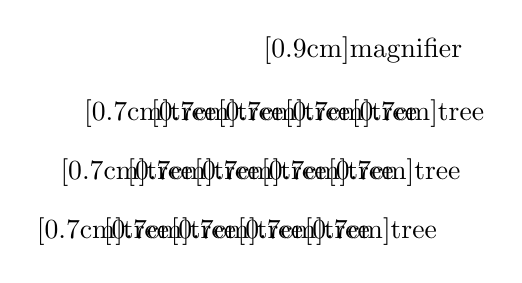
\begin{tikzpicture}
        \foreach \x in {0,...,4}{\foreach \y in {0,...,2}{\node at (\x*0.85+0.3*\y, \y*0.75) {\bigemoji[0.7cm]{tree}};}}
        \node at (3.3,2.3) {\bigemoji[0.9cm]{magnifier}};
      \end{tikzpicture}\par\smallskip
      {\small Սկաներով այն փնտրելը նույնն է, թե անտառում փնտրես \textbf{մի կոնկրետ ծառ}}}
    \end{column}
  \end{columns}
\end{frame}

% Three techniques, one reason: we want to be liked
\begin{frame}{Երեք հնարք, մեկ պատճառ}
  \begin{tikzpicture}[x=1cm, y=1cm]
    \foreach \i/\c/\n/\r/\s in {
        0/butter/{Ոտքը դռան արանքում}/{Համաձայնել ես։ Հաջորդ նման խնդրանքը մերժելը կհիասթափեցնի ու կփչացնի կարծիքը քո մասին}/1,
        1/brainpink/{Դուռը երեսին}/{Մերժել ես մեծը ու գիտես, որ դիմացինը քեզ դրա համար չի սիրի։ Փոքրին համաձայնում ես որպես «մխիթարանք»}/2,
        2/lavender/{Ցածր գնդակ}/{Արդեն համաձայնել ես։ Հետ կանգնելը կհիասթափեցնի ու քեզ վատ ցույց կտա}/3}{
      \node[personnode, fill=\c!55!cardwhite, text width=3.2cm, minimum height=1.15cm, font=\blackfont\small, visible on=<\s->]
        (t\i) at (0,-\i*1.38) {\n};
      \node[personnode, text width=8.6cm, minimum height=1.15cm, anchor=west, align=left, visible on=<\s->]
        (r\i) at (2.6,-\i*1.38) {\r};
      \draw[-{Stealth[length=2.5mm]}, plum, line width=1pt, visible on=<\s->] (t\i) -- (r\i);}
  \end{tikzpicture}\par\vspace{3mm}
  \onslide<4->{%
  \begin{card}[colback=butter!45!cream]
    Երեքն էլ օգտագործում են մեր ցանկությունը, որ մեր մասին \textbf{լավ մտածեն}։ Այն այնքան ուժեղ է, որ հաղթում է տրամաբանությանը։
  \end{card}}
\end{frame}

% Consistency, reciprocity, dominance
\begin{frame}{Եվս երեք պատճառ}
  \begin{columns}[T]
    \begin{column}{0.32\textwidth}
      \begin{card}[colback=butter!45!cream]
        \centering\bigemoji[0.8cm]{link}\par\smallskip
        \raggedright{\blackfont Հետևողականություն}\par
        Արդեն փող տվել ես, ուրեմն ուղեղը որոշում է, որ \textbf{ուզում ես} էլի տալ։ Այլապես դիսոնանս է
      \end{card}
    \end{column}
    \begin{column}{0.32\textwidth}
      \onslide<2->{%
      \begin{card}[colback=mint!35!cardwhite]
        \centering\bigemoji[0.8cm]{handshake}\par\smallskip
        \raggedright{\blackfont Փոխադարձություն}\par
        Փոքր խնդրանքը մեծից հետո ուղեղը ընկալում է որպես լավություն, որովհետև \textbf{ապուշ է}
      \end{card}}
    \end{column}
    \begin{column}{0.32\textwidth}
      \onslide<3->{%
      \begin{card}[colback=lavender!40!cardwhite]
        \centering\bigemoji[0.8cm]{crown}\par\smallskip
        \raggedright{\blackfont Գերիշխանություն}\par
        Հետ կանգնես՝ նշանակում է, որ նա քեզ կառավարեց։ Ո՛չ, կանես, որովհետև \textbf{բարի ես, անիծյալ}
      \end{card}}
    \end{column}
  \end{columns}
\end{frame}

% Summary of the section
\begin{frame}{Ուղեղը մեզ հեշտ թիրախ է դարձնում}
  \begin{columns}[c]
    \begin{column}{0.56\textwidth}
      Ուղեղը ստիպում է, որ ուզենք\par\smallskip
      \begin{enumerate}
        \item<1-> որ մեզ \textbf{սիրեն}
        \item<2-> լինել \textbf{վերևում}
        \item<3-> լինել \textbf{հետևողական}
      \end{enumerate}
      \vspace{2mm}
      \onslide<4->{Արդյունքում խոցելի ենք ամեն անսկզբունք մարդու առաջ, ով ուզում է մեր փողը ու մի քիչ սակարկել գիտի։\par}
    \end{column}
    \begin{column}{0.4\textwidth}
      \onslide<5->{%
      \begin{bookquote}
        Անհավանական բարդ օրգան է պետք, որպեսզի \textbf{այսքան հիմար} բան անի։
      \end{bookquote}
      \centering\mascot[2cm]{confused}}
    \end{column}
  \end{columns}
\end{frame}

% First half on one page
\begin{frame}{Առաջին կեսը՝ մեկ էջում}
  \begin{columns}[T]
    \begin{column}{0.31\textwidth}
      \begin{card}[colback=peach!35!cardwhite]\emoji{hug}\ {\blackfont Ուրիշ մարդիկ}\par Խմբեր կազմում են անգամ ապստամբները. շփումը պարտադիր է\end{card}
    \end{column}
    \begin{column}{0.31\textwidth}
      \begin{card}[colback=mint!35!cardwhite]\emoji{masks}\ {\blackfont Դեմքեր ու խոսք}\par Լեզուն ցրված է ողջ ուղեղով, իսկ դեմքը մատնում է այն, ինչ բառերը թաքցնում են\end{card}
    \end{column}
    \begin{column}{0.31\textwidth}
      \begin{card}[colback=butter!45!cream]\emoji{carrot}\ {\blackfont Համոզում}\par Երեք հնարքն էլ աշխատում են, որովհետև ուզում ենք, որ մեզ սիրեն\end{card}
    \end{column}
  \end{columns}
  \vspace{2mm}
  \centering
  \mascot[1.2cm]{happy}\par
  {\small Հարցեր կա՞ն մինչև ընդմիջումը}
\end{frame}

% ---------------------------------------------------------------- break
\begin{frame}[plain]
  \begin{tikzpicture}[remember picture, overlay]
    \fill[butter!60!cream] (current page.south west) rectangle (current page.north east);
    \node at ([yshift=8mm]current page.center) {\mascot[4cm]{sleepy}};
    \node[anchor=north, font=\titlefont\fontsize{30}{32}\selectfont, text=plum] at ([yshift=-17mm]current page.center) {Ընդմիջում};
    \node[anchor=north, font=\mediumfont\large, text=plum] at ([yshift=-31mm]current page.center)
      {5 րոպե \emoji{coffee}\quad Կանգնիր, ձգվիր, ջուր խմիր};
  \end{tikzpicture}
\end{frame}
